% !TEX TS-program = pdflatex
% !TEX encoding = UTF-8 Unicode

\documentclass[11pt]{article}
\usepackage[utf8]{inputenc} 
\usepackage[parfill]{parskip}
\usepackage[T1]{fontenc} 

\usepackage{polski}
\usepackage{float}
\usepackage{fixltx2e}
\usepackage{calc}
\usepackage[export]{adjustbox} % also loads graphicx
\usepackage{makeidx}
\usepackage{multicol}
\usepackage{multirow}
\PassOptionsToPackage{warn}{textcomp}
\usepackage{textcomp}
\usepackage[nointegrals]{wasysym}
\usepackage[table]{xcolor}

\usepackage{csvsimple}

% Font selection
\usepackage[T1]{fontenc}
\usepackage[scaled=.90]{helvet}
\usepackage{courier}
\usepackage{amssymb}
\usepackage{sectsty}

%%% PAGE DIMENSIONS
\usepackage{geometry} % to change the page dimensions
\geometry{a4paper} % or letterpaper (US) or a5paper or....
\geometry{margin=1in} % for example, change the margins to 2 inches all round

\usepackage{graphicx} % support the \includegraphics command and options
\usepackage[parfill]{parskip} % Activate to begin paragraphs with an empty line rather than an indent

%%% PACKAGES
\usepackage{booktabs} % for much better looking tables
\usepackage{array} % for better arrays (eg matrices) in maths
\usepackage{paralist} % very flexible & customisable lists (eg. enumerate/itemize, etc.)
\usepackage{verbatim} % adds environment for commenting out blocks of text & for better verbatim
\usepackage{subfig} % make it possible to include more than one captioned figure/table in a single float
% These packages are all incorporated in the memoir class to one degree or another...
\usepackage{graphicx} 
\graphicspath{ {../analysis/} }

\usepackage{ifpdf}
\ifpdf
\usepackage[pdftex,pagebackref=true]{hyperref}
\else
\usepackage[ps2pdf,pagebackref=true]{hyperref}
\fi
\hypersetup{%
	colorlinks=true,%
	linkcolor=blue,%
	citecolor=blue,%
	unicode%
}


%%% HEADERS & FOOTERS
\usepackage{fancyhdr} % This should be set AFTER setting up the page geometry
\pagestyle{fancy} % options: empty , plain , fancy
\renewcommand{\headrulewidth}{0pt} % customise the layout...
\lhead{}\chead{}\rhead{}
\lfoot{}\cfoot{\thepage}\rfoot{}
%%% END Article customizations

%%% The "real" document content comes below...

\title{PSZT - Uczenie Maszynowe}
\author{Stawczyk Przemysław 293153, Piotr Zmyślony 268833}
\date{} % Activate to display a given date or no date (if empty),
% otherwise the current date is printed 

\begin{document}
	\maketitle
	\setcounter{secnumdepth}{3}
	\setcounter{tocdepth}{3}
	\tableofcontents
	\clearpage
\section{Opis zagadnienia}
\subsection{Treść zadania}
Przedstawić wyniki analizy zbioru \textsl{Bankruptcy}, opisać procedurę eksperymentalną uczenia maszynowego z wykorzystaniem algorytmów \textsl{random forest} i \textsl{k-najbliższych sąsiadów} oraz opisać wyniki strojenia parametrów powyższych algorytmów.
\subsection{Narzędzia}
Skrypty oraz algorytm zostały zaimplementowane w Pythonie 3. Wykorzystano biblioteki: \textsl{imblearn.over\_sampling.SMOTE, sklearn, numpy, matplotlib, scipy.io, impyute}.
\section{Opis preprocesingu i modelowania}
\subsection{Opis danych wejściowych}
Jako dane wejściowe posiadamy 5 plików \textsl{.arff}, z których każdy zawiera ekonomiczne wskaźniki z systemu EMIS na temat polskich firm i ich klasyfikację względem tego, czy firmy zbankrutowały po \textsl{n} latach od roku, w którym zostały zebrane dane. Liczba \textsl{n} lat jest różna dla każdego z plików, od 1 do 5, a każda firma opisana jest przez 64 atrybuty, od \textsl{X1} do \textsl{X64}.
\subsection{Analiza zbioru danych}
\subsubsection{Brakujące dane}
Zaczęliśmy od analizy brakujących danych w wierszach. Jak widać w poniższych wynikach w większości zbiorów około połowa wierszy ma brakujące pola.
\begin{center}
\begin{tabular}{|c|m{0.7in}|m{0.7in}|m{0.7in}|m{0.7in}|m{0.7in}|}
	\hline
	& \textit{1 rok} & \textit{2 lata} & \textit{3 lata} & \textit{4 lata} & \textit{5 lat} \\ \hline
	\textit{długość} & 7027 & 10173 & 10503 & 9792 & 5910 \\ \hline
	\textit{pełne wiersze} & 3194 & 4088 & 4885 & 4769 & 3031 \\ \hline
	\textit{wiersze wybrakowane} & 3833 & 6085 & 5618 & 5023 & 2879 \\ \hline
\end{tabular}
\end{center}
Następnie przeprowadziliśmy analizę rozkładu brakujących danych w kolumnach i wierszach korzystając z biblioteki pythona \textit{missingno} [Rys. 1-5]\\

\begin{figure}[h]
\caption{1 rok}
	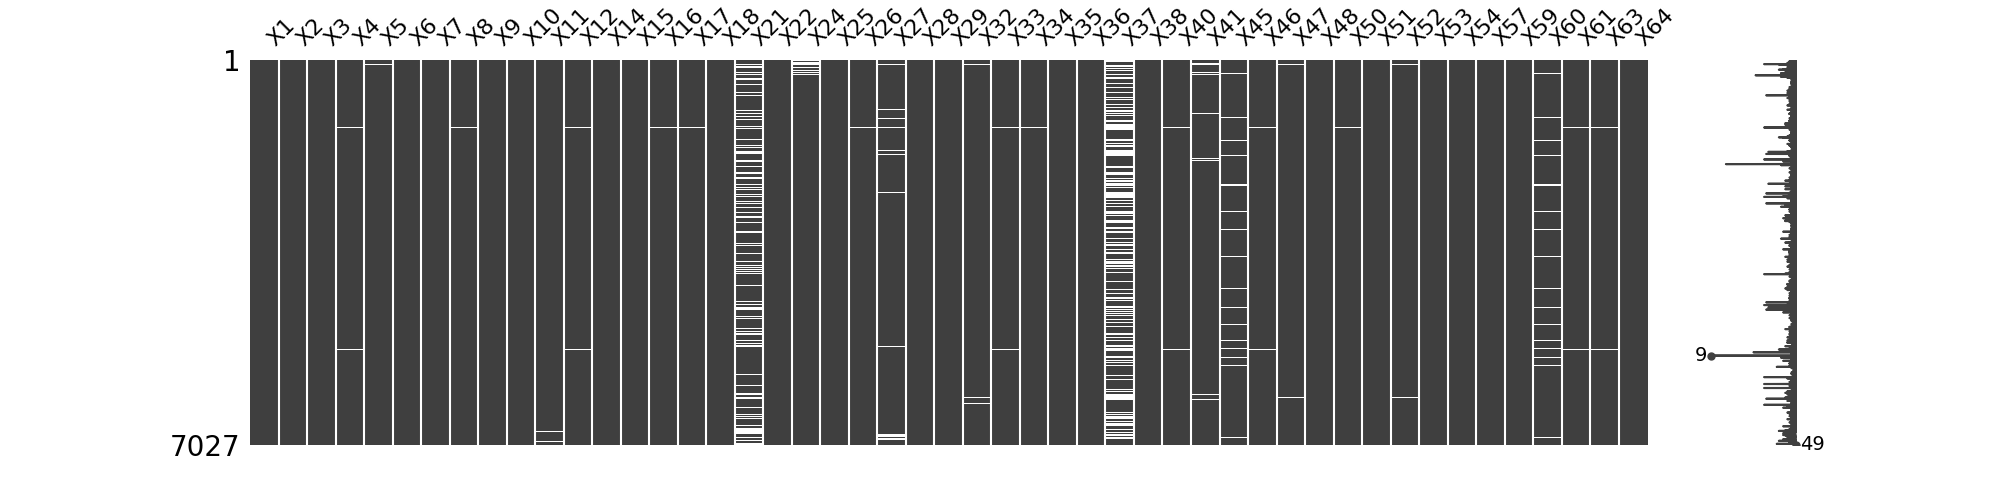
\includegraphics[width=\textwidth]{year_1}
\end{figure}
\begin{figure}[p]
\caption{2 lata}
	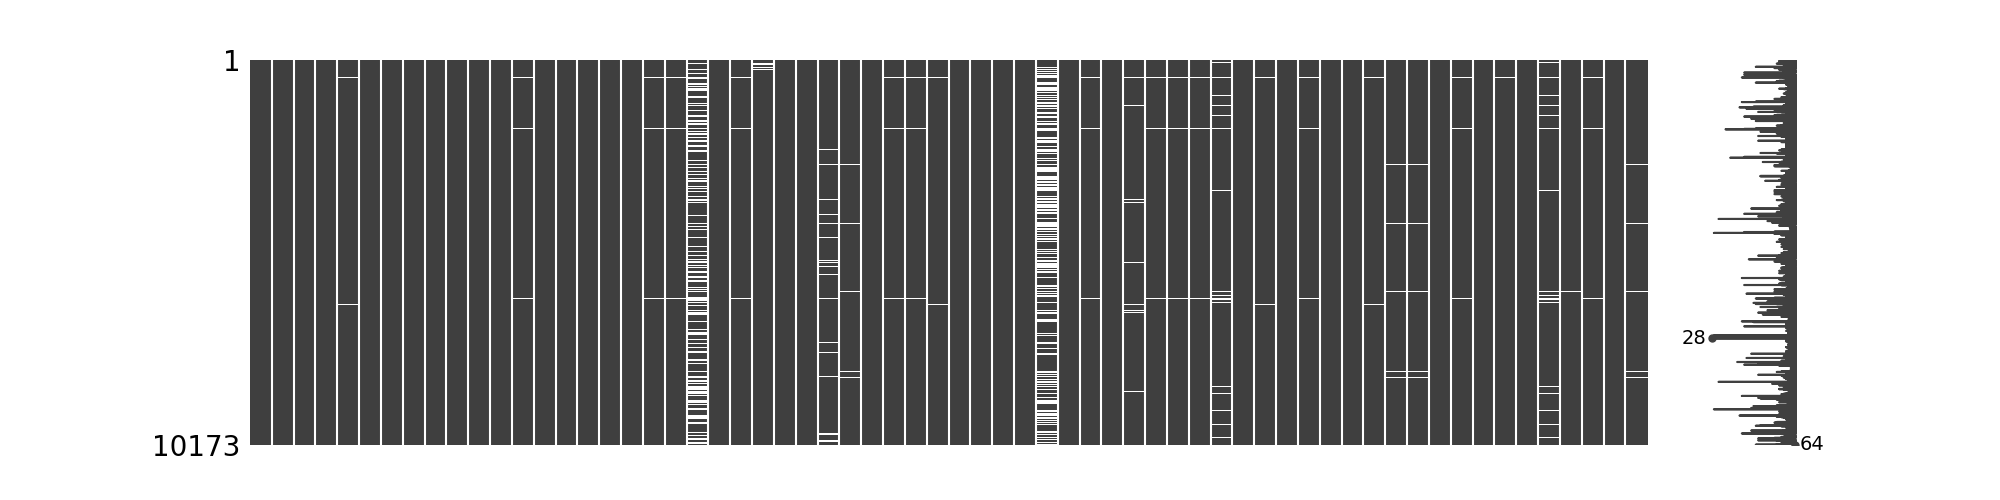
\includegraphics[width=\textwidth]{year_2}
\caption{3 lata}
	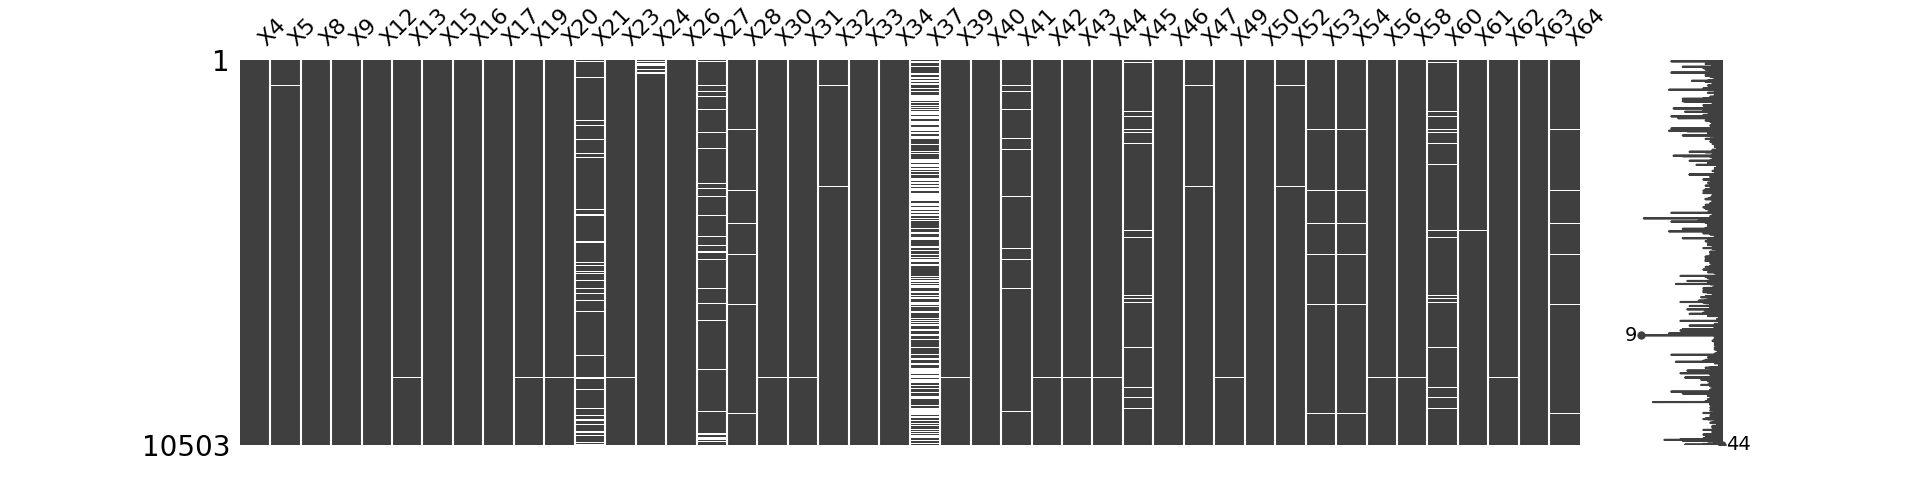
\includegraphics[width=\textwidth]{year_3}
\caption{4 lata}
	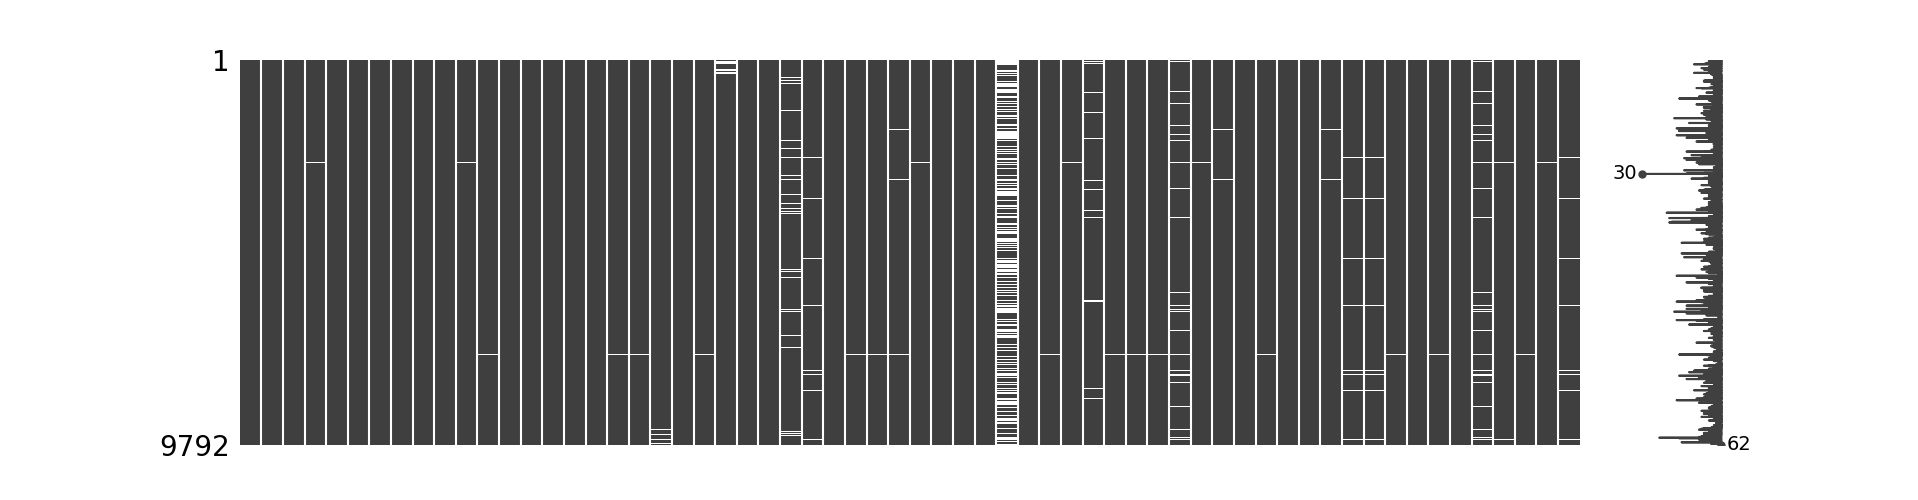
\includegraphics[width=\textwidth]{year_4}
\caption{5 lat}
	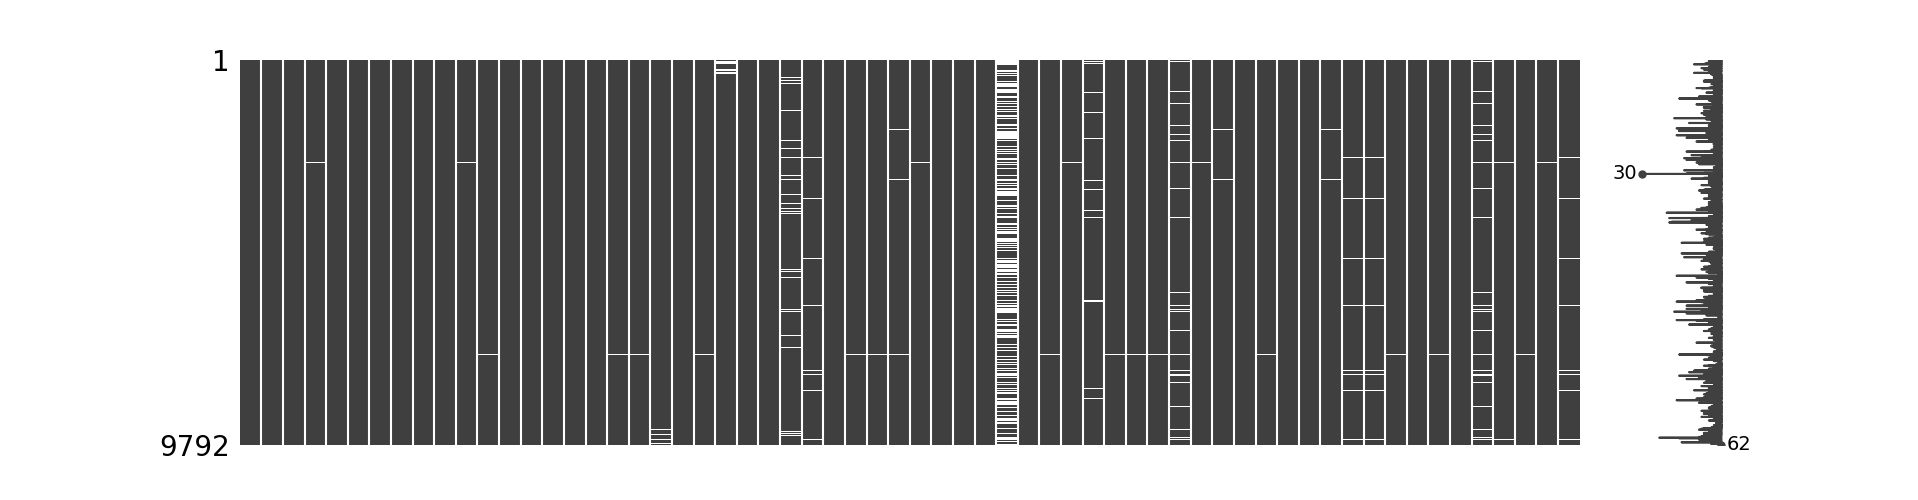
\includegraphics[width=\textwidth]{year_5}
\end{figure}

Jak widać większość brakujących danych jest w kolumnie \textit{X37}. Kolumna \textit{X21} ma brakujące w niektórych ale nie wszystkich latach.\\
Trudno nam było ocenić jaki charakter mają braki w tych danych, czy są skorelowane w wartościami w innych kolumnach czy zupełnie losowe. Wierszy z brakującymi danymi jest około połowy lub więcej. Aby nie odrzucać tak dużej liczby krotek zdecydowaliśmy się interpolować brakujące dane.\\
W tym celu wybraliśmy 4 metody:
\begin{enumerate}
	\item Wstawianie średniej w danej kolumnie \textit{(Jako punkt odniesienia)}
	\item K najbliższych krotek
	\item Spodziewanej Maksymalizacji \textit{(Expected Maximalisation)}
	\item Algorytm MICE
\end{enumerate}
\subsubsection{Zbalansowanie danych}
Dokonaliśmy analizy ile z poszczególnych rekordów należy do klas klasyfikacyjnych
\begin{center}
	\begin{tabular}{|c|m{0.7in}|m{0.7in}|m{0.7in}|m{0.7in}|m{0.7in}|}
		\hline
		\textit{Czy zbankrutowano:}& \textit{rok 1} & \textit{rok 2} & \textit{rok 3} & \textit{rok 4} & \textit{rok 5} \\ \hline
		\textit{Nie} & 6756 & 9773 & 10008 & 9277 & 5500 \\ \hline
		\textit{Tak} & 271 & 400 & 495 & 515 & 410 \\ \hline \hline
		\textit{procent większości} & 3.857 \% & 3.932 \% & 4.713 \% & 5.259 \% & 6.937 \% \\ \hline
	\end{tabular}
\end{center}
Dane w zbiorach są mocno niezbalansowane dlatego zdecydowaliśmy się na interpolację korzystając z metody \textit{SMOTE (Synthetic Minority Over Sampling Technique)}
\subsection{Przepływ Danych}
Po powyższej analizie zdecydowaliśmy o następującym przepływie oryginalnych danych do konstrukcji modeli.\\
Walidacji modeli planujemy dokonać korzystając K-krotnej walidacji krzyżowej.
\subsubsection{Wizualizacja Przepływu Danych}
\begin{figure}[h]
	\caption{Przepływ Danych}
	\begin{center}
		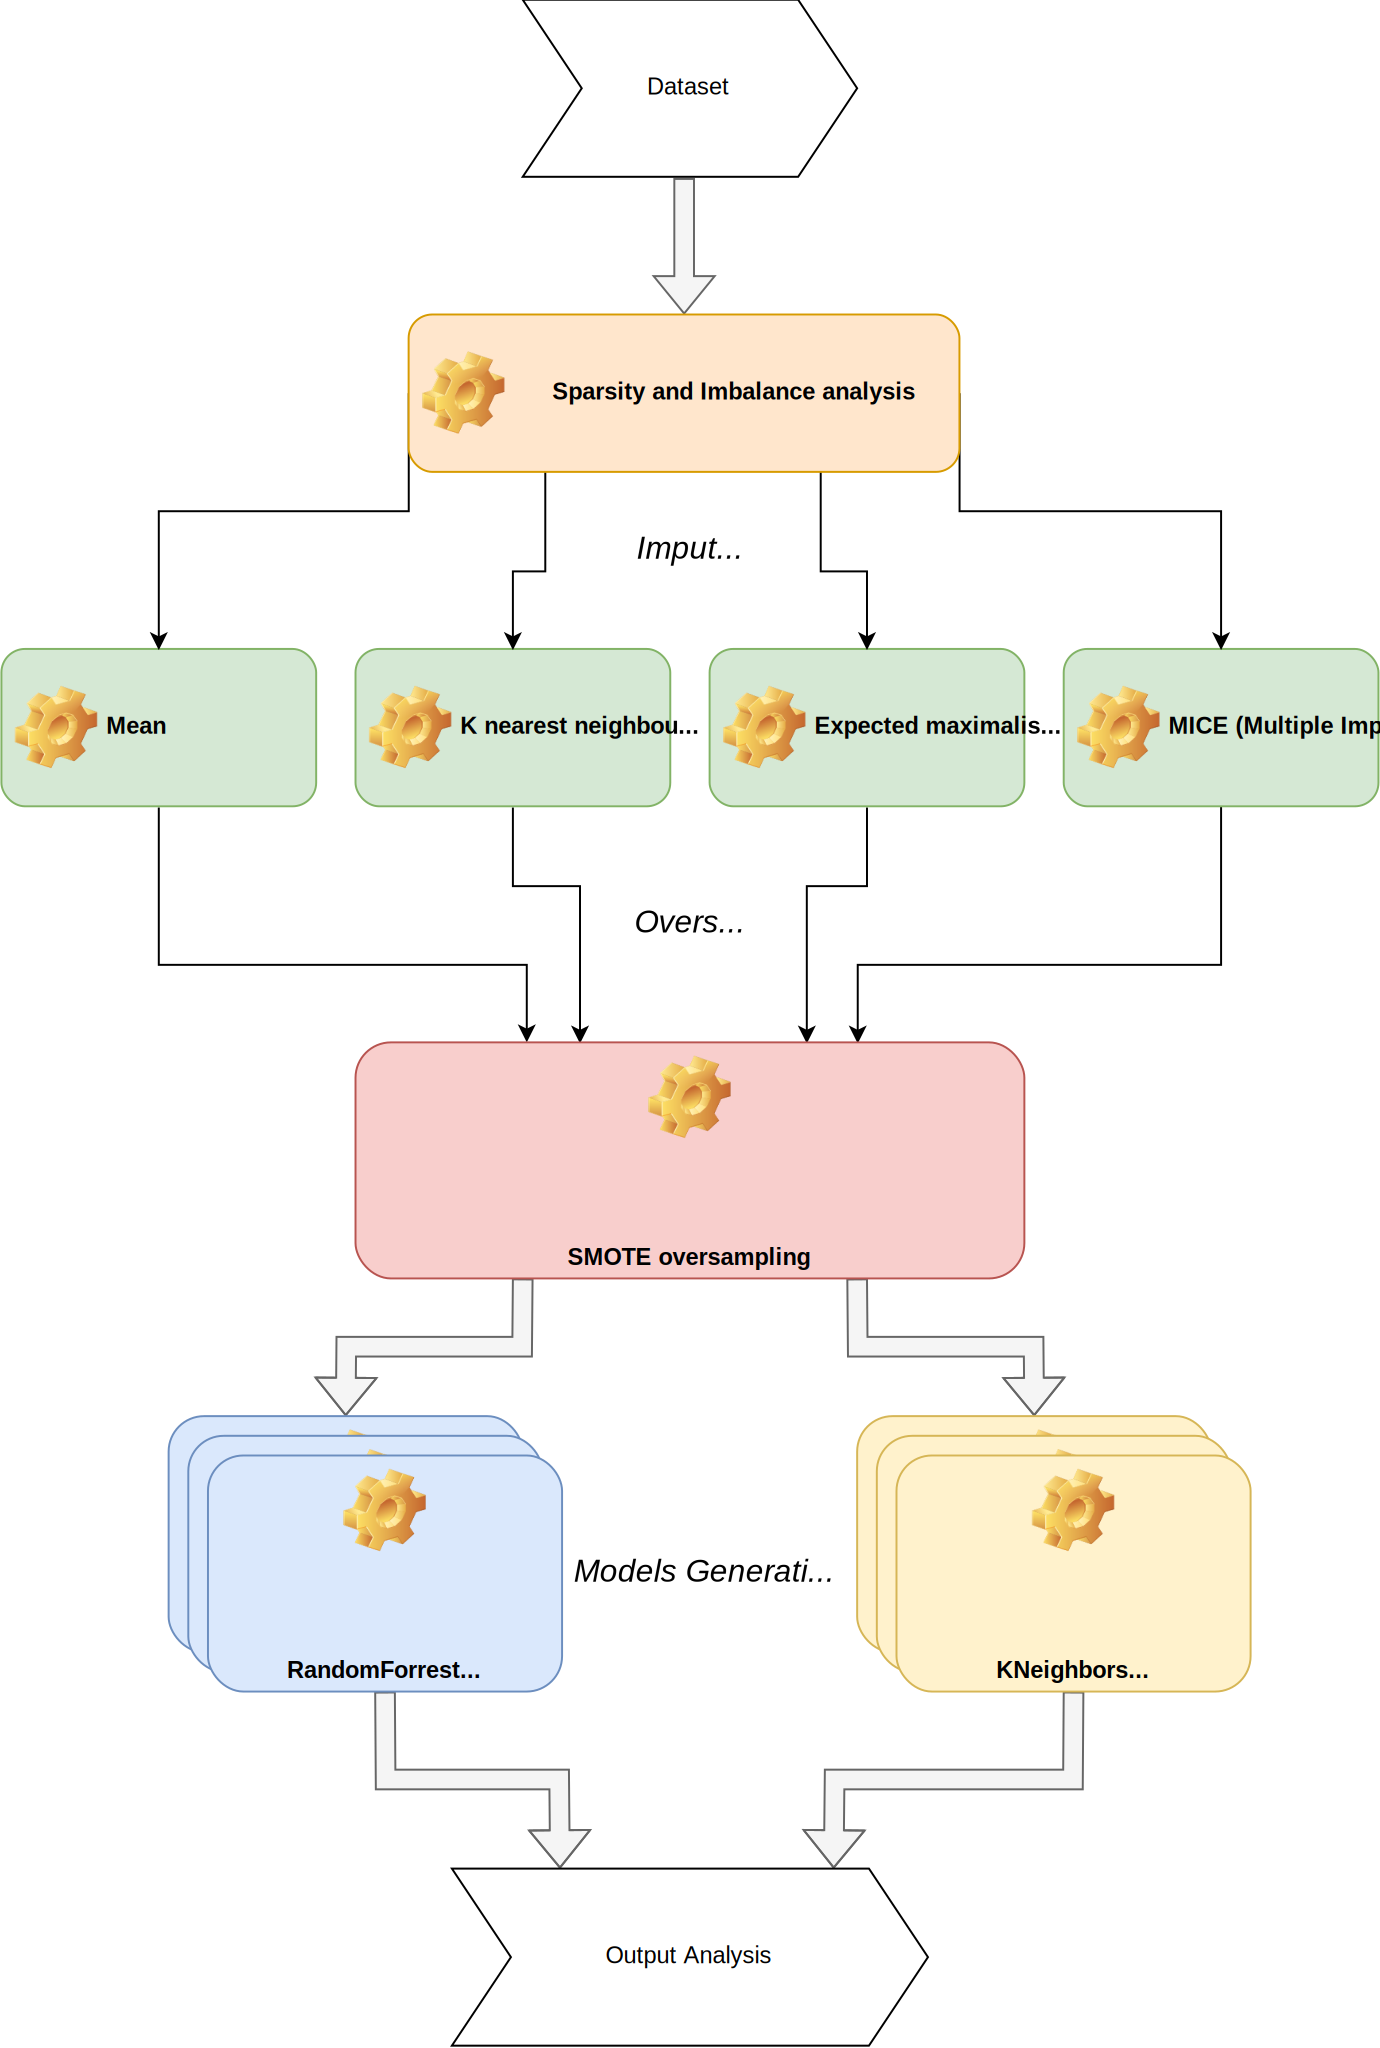
\includegraphics[width=4in]{Dataflow}
	\end{center}
\end{figure}
\section{Modele}
Zgodnie z poleceniem wykorzystaliśmy algorytmy tworzenia modeli : 
\begin{itemize}
	\item Las Losowy \textit{[RF - Random Forrest]}
	\item K Najbliższych sąsiadów \textit{[KNN - K Nearest Neighbors]}
\end{itemize}
Implementacje wymienionych algorytmów pochodzą z biblioteki \textit{sklearn}.
\subsection{Parametry Modeli}
W początkowej fazie porównywania modeli chcieliśmy zbadać, który klasyfikator (KNN czy Random Forest) daje ogólnie lepsze wyniki. Z tego początku parametry dobierane były ręcznie, tak aby utworzyć zestawienie pokazujące różnice między tymi dwoma klasyfikatorami (Rysunek \ref{knn_vs_rf}) oraz porównać wpływ zmiany niektórych parametrów na rezultat końcowy dopasowywania modeli.



Później, po ustaleniu, że Random Forest jest znacznie klasyfikatorem dla tego problemu, użyliśmy wyszukiwania na hipersiatce, tak aby program sam znalazł hiperparametry dla tego modelu.
 
\section{Wyniki Eksperymentu}
\subsection{Porównanie klasyfikatorów}
Początkowo, sprawdziliśmy jaka ilość sąsiadów w metodzie KNN daje najlepszy model, co zademonstrowane jest na Rys. \ref{knn_varied_n_neighbors}. Zaobserwowaliśmy, że nasz model najlepiej dopasowywał się jeśli za najbliższego sąsiada uznawany był tylko jeden punkt.
Wynik dopasowania każdego klasyfikatora uzyskiwaliśmy dzięki 5-krotnej walidacji krzyżowej.
\begin{figure}[H]
\caption{Porównianie liczby K najbliższych sąsiadów}
\label{knn_varied_n_neighbors}
\centering
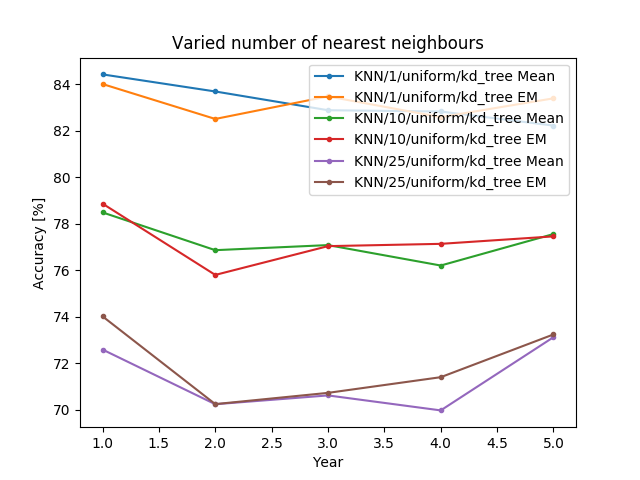
\includegraphics[scale=0.8]{knn_varied_n_neighbors}
\end{figure}

Okazuje się, że klasyfikator Random Forest sprawdza się znacznie lepiej niż najlepszy model klasyfikatora KNN. Porównanie dla tych modeli znajduje się na Rys. \ref{bestknn_vs_bestrf}.
\begin{figure}[H]
\caption{Porównianie KSS i RF}
\label{bestknn_vs_bestrf}
\centering
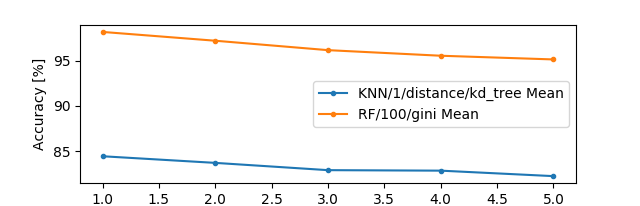
\includegraphics[scale=0.8]{bestknn_vs_bestrf}
\end{figure}
\subsection{Metoda interpolowania brakujących danych}
Na Rys. \ref{why_knn_imput_sucks} możemy zaobserwować różnicę w precyzji modeli, zależnie od typu wstawiania danych - zwykłe wstawianie wartości uśrednianej osiąga wynik lepszy niż metoda uzupełniania danych poprzez wstawianie średniej k najbliższych sąsiadów.
\begin{figure}[H]
\caption{Porównianie metod wstawiania danych}
\label{why_knn_imput_sucks}
\centering
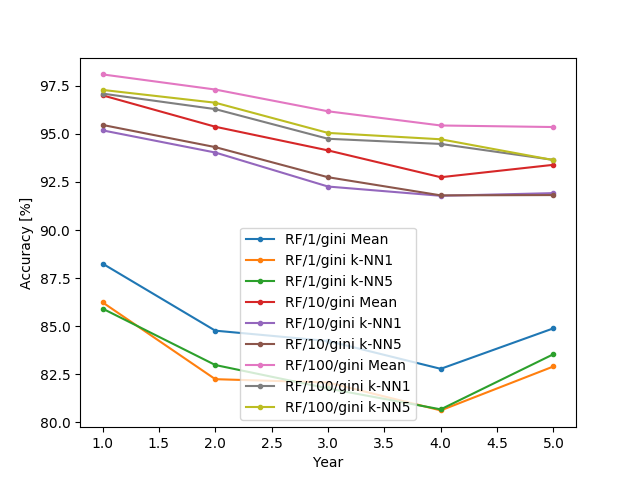
\includegraphics[scale=0.8]{why_knn_imput_sucks}
\end{figure}
Okazuje się, że metoda Mean jest również lepsza niż EM, co obrazuje Rys. \ref{rf_varied_n_trees_entropy}. Można stąd wnioskować, że wpływ najbardziej wybrakowanych kolumn \textit{X37} i \textit{X21} na potencjalny, przyszły status bankructwa jest znikomy.
Stąd, do liczenia najlepszych hiperparametrów zastosowaliśmy tylko metodę wstawiania wartości średnich.
\begin{figure}[H]
\caption{Porównianie metod wstawiania danych}
\label{rf_varied_n_trees_entropy}
\centering
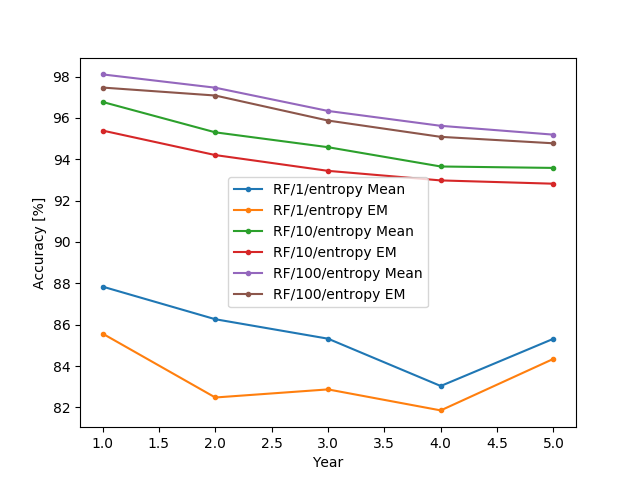
\includegraphics[scale=0.8]{rf_varied_n_trees_entropy}
\end{figure}
\subsection{Parametry dobrane przez hipersiatkę}
Hiperparametry dobierane były generując dla każdego z pięciu zestawów danych po 72 klasyfikatory (stosując 5-krotną walidację krzyżową było ich w sumie 360) i później wybierając ten, który dawał najlepszy odsetek prawidłowych klasyfikacji na zbiorach testowych.

Zmieniane hiperparametry modelu klasyfikatora to: \textsl{n\_estimators} (ilość drzew decyzyjnych), \textsl{criterion} (sposób na który drzewa podejmują decyzje), \textsl{max\_features} (maksymalna liczbę funkcji do rozważenia podczas szukania podziału), \textsl{max\_depth} (maksymalna głębokość drzewa). Poniżej, w tabeli, jest lista wszystkich testowanych parametrów:

\begin{center}
	\begin{tabular}{|c|c|c|c|}
		\hline
		\textit{n\_estimators}& \textit{criterion} & \textit{max\_features} & \textit{max\_depth}\\ \hline
		1, 10, 100 & "gini", "entropy" & "auto", "log2", 16 & 10, 100, 1000, None \\ \hline
	\end{tabular}
\end{center}

Otrzymaliśmy następujące rezultaty dla kolejnych ilości lat:

\begin{center}
	\begin{tabular}{|c|c|c|c|c|c|}
		\hline
		& \textbf{1 rok} & \textbf{2 lata} & \textbf{3 lata} & \textbf{4 lata} & \textbf{5 lat} \\ \hline
		\textit{n\_estimators} & 100 & 100 & 100 & 100 & 100 \\ \hline
		\textit{criterion} & entropy & entropy & gini & entropy & entropy \\ \hline
		\textit{max\_features} & log2 & auto & log2 & 16 & 16 \\ \hline
		\textit{max\_depth} & 100 & None & None & 100 & 100 \\ \hline
	\end{tabular}
\end{center}

Widzimy, że tak twierdzi teoria - za każdym razem została wybrana największa ilość estymatorów, a reszta parametrów wahała się zależnie od analizowanego zbioru danych. 

Efekt działania przeszukiwania hipersiatki - modele o najlepiej dobranych hiperparametrach z podanych zbiorów, są widoczne na Rys. \ref{best_rf}.

Prawdopodobnie uzyskanie lepszego wyniku byłoby możliwe analizując więcej hiperparametrów o większym zakresie dostępnych ustawień, jednak jesteśmy ogranieczeni przez moc obliczeniową naszych urządzeń.

\begin{figure}[H]
\caption{Precyzja modeli dopasowanych hipersiatką}
\label{best_rf}
\centering
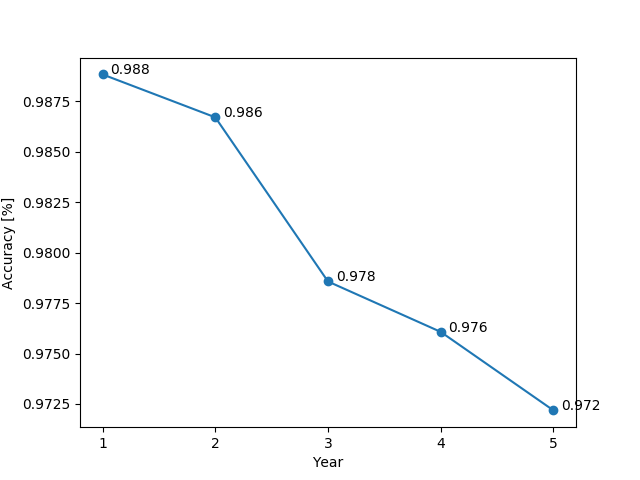
\includegraphics[scale=0.8]{best_rf}
\end{figure}
\subsection{Interpretacja}
% jakiś komentarz do obrazków powyżej jeśli nie bezpośrdenio pod nimi ???
% wnioski że najlepszy np Las Losowy z tymi paramsami i imputerem Xd
Możemy zauważyć spadek poprawności klasyfikacji firm wraz z wydłużaniem się okresu prognozowania, co jest dosyć oczywistym faktem, ponieważ przewidywanie przyszłości jest coraz trudniejsze dla coraz bardziej oddalonych w czasie sytuacji. Stąd też większe prawdopodobieństwo, że firma której się powodzi zbankrutuje w okresie 5 lat, niż nagle, po upływie roku.
\end{document}
